\documentclass{standalone}
\usepackage{tikz}
\usepackage{ctex,siunitx,upgreek}
\usepackage{tkz-euclide}
\usepackage{amsmath}
\usetikzlibrary{patterns, calc}
\usetikzlibrary {decorations.pathmorphing, decorations.pathreplacing, decorations.shapes,}
\begin{document}
\small
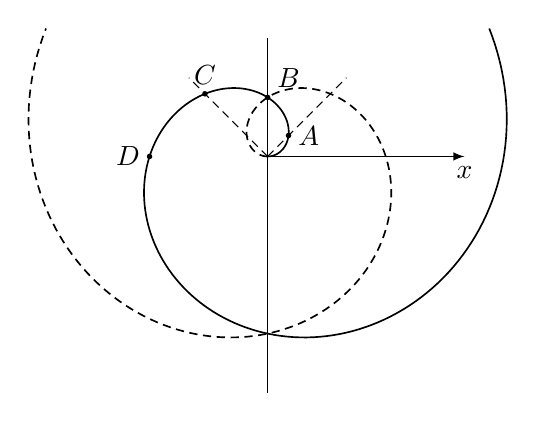
\begin{tikzpicture}[>=latex,scale=0.5]
  \draw[thin,->](0,0)--(5,0)node[below]{$x$};
  \draw[thin](0,-6)--(0,3);
  \draw[semithick,domain=0:390,samples=200] plot (\x:{3*\x/180});
  \draw[semithick,densely dashed,domain=0:390,samples=200] plot (-\x:{-3*\x/180});
  \fill(45:0.75)circle(2pt)node[right]{$A$};
  \fill(90:1.5)circle(2pt)node[above right]{$B$};
  \fill(135:2.25)circle(2pt)node[above]{$C$};
  \fill(180:3)circle(2pt)node[left]{$D$};
  \draw[thin,densely dashed] (0,0)--(2,2)(0,0)--(-2,2);
\end{tikzpicture}
\end{document}